%% ============================================================
%% chapters/chapter3_openpass.tex
%% Chapter 3: OpenPASS — Characterizing Far-Edge AI Deployment
%% Failures in Digital Agriculture
%% ============================================================

\chapter{OpenPASS: Characterizing Far-Edge AI Deployment Failures in Digital Agriculture}
\label{ch:openpass}

%% ============================================================
\section{When the Field Rewrites the Spec}
\label{sec:ch3_intro}
%% ============================================================
Digital agriculture has a timing problem. Crop stress, pest infestation, and nutrient deficiency do not wait for a convenient connectivity window. The value of an aerial survey is in the analysis it produces during or immediately after the mission, while the flight crew is still on-site and can act. A system that uploads raw imagery to a cloud backend for processing, waits for results, and returns them hours later delivers information that is correct but no longer actionable. The window has closed.

This constraint drives a straightforward architectural requirement: inference must happen at the field edge, on the hardware that made the flight, without a cloud round-trip. The UAV captures imagery, the edge node processes it, and the farmer receives crop health analysis before the mission ends. No external network is required, and none should be assumed.

OpenPASS was built to satisfy exactly this requirement. It is a containerized AI application running on K3S, a lightweight single-binary Kubernetes distribution, that performs crop health inference on drone-captured aerial imagery entirely at the field edge. The edge node is a standard x86\_64 field laptop. The drone is a UAV platform capturing high-resolution aerial imagery. The pipeline moves from flight to orthomosaic to crop health analysis without touching external infrastructure. The intelligence is at the field level. That was the design intent.

What the design intent did not account for was the field itself. The first real-world deployment of OpenPASS outside a controlled lab environment took place at a soybean farm in Stoutsville, Ohio, in summer 2025. The system that had been tested extensively in the lab, where infrastructure assumptions went unquestioned, met a physical environment that honored none of them. Three failures surfaced, each rooted in a different assumption the platform had never been asked to question.

This chapter documents those failures, explains why they were structural rather than incidental, and describes the architectural solutions that resolved each one. The framework that emerges from this analysis, what we call the inflection-point classification, is the chapter's primary contribution. It is a way of thinking about far-edge deployment failures that makes them tractable: nameable, documentable, and addressable before the next system ships.

%% ============================================================
\section{What Came Before: Edge Orchestration and Its Assumptions}
\label{sec:ch3_arch}
%% ============================================================
Container orchestration for edge environments is an active research area, and several platforms have emerged to address it. Understanding where they succeed and where they fall short is necessary context for understanding what OpenPASS had to solve.

KubeEdge extends Kubernetes to the edge by splitting the control plane: cloud-side components handle scheduling and state synchronization, while a lightweight EdgeCore agent runs workloads on the edge node \cite{xiong2018kubeedge}. The architecture explicitly accommodates intermittent connectivity through local metadata caching. In practice, however, KubeEdge's offline tolerance is conditional. The edge node can continue running existing workloads through a disconnection. What it cannot do is reconstruct a failed pod without reconnecting to the cloud-side control plane. When a container crashes and the node is offline, recovery requires the node to come back online, a requirement that is documented in the project's own issue tracker and fundamentally incompatible with far-edge environments where extended disconnection is the norm, not the exception.

OpenYurt takes a similar architectural approach, tunneling Kubernetes control plane communication through a cloud-edge proxy layer and adding autonomy features for disconnected edge nodes \cite{yakubov2025comparative}. Like KubeEdge, it tolerates disconnection for running workloads but does not support complete self-sufficient reconstruction without cloud coordination.

K3S vanilla is the closest to what OpenPASS is built on. K3S is a lightweight Kubernetes distribution packaged as a single binary with an embedded SQLite datastore, designed for resource-constrained edge hardware \cite{k3sdocs2024}. Out of the box, it uses Flannel as its CNI plugin with a VXLAN backend. It supports private registry mirroring via configuration. It runs well on x86\_64 hardware. What it does not do is account for enterprise network environments that block the UDP ports Flannel requires, or for deployment sites with zero internet access, or for startup resource contention on constrained hardware under real field load. Those problems exist in its documentation as known requirements and warnings, not as solved problems \cite{k3sdocs2024}.

MicroK8s is a single-node Kubernetes distribution from Canonical aimed at developer workstations and IoT. It is not designed for far-edge deployment and has no documented path to offline-first operation.

Eclipse ioFog provides an edge microservice platform with a ComSat networking component that can buffer data during disconnection and handle NAT traversal without VPN configuration \cite{iofog2019eclipse}. It is more network-aware than standard Kubernetes distributions, but its offline capability is buffering and queuing, not self-sufficient operation. It still depends on a centralized Controller for microservice orchestration.

Boubin et al. characterize the resource management constraints that arise when AI inference and flight control compete for compute on fully autonomous aerial systems at the edge, establishing that co-locating these workloads on a single constrained node produces resource contention and scheduling failures that standard cloud-oriented orchestration platforms do not address \cite{boubin2019managing}.

The pattern across all of these systems is consistent and important. Each one treats network connectivity as the normal operating state. Offline behavior, where it exists at all, is a degraded mode, a temporary condition the system tolerates until connectivity is restored. None of them was designed with the premise that connectivity might never exist during a mission. None has been deployed in a real agricultural field and documented what broke.

\begin{table}[htbp]
\centering
\small
\caption{Far-edge deployment capability comparison. \cmark~=~full support; \pmark~=~partial; \xmark~=~not supported; \namark~=~out of scope. OpenPASS extends K3s (vanilla) with solutions for all three far-edge deployment gaps identified at Stoutsville.}
\label{tab:edge_capability_comparison}
\renewcommand{\arraystretch}{1.4}
\begin{tabularx}{\textwidth}{lXXXXX}
\hline
\textbf{System}
  & \textbf{\makecell{Offline\\Pod\\Reconstruction}}
  & \textbf{\makecell{Firewall-\\Tolerant\\CNI}}
  & \textbf{\makecell{Single-Node\\Far-Edge\\Optimized}}
  & \textbf{\makecell{No Cloud\\Control Plane}}
  & \textbf{\makecell{Disconnected\\Field\\Validated}} \\
\hline
\textbf{OpenPASS} (ours)  & \cmark & \cmark & \cmark & \cmark & \cmark \\
K3s (vanilla)             & \xmark & \xmark & \cmark & \cmark & \xmark \\
\hline
KubeEdge~\cite{xiong2018kubeedge}       & \pmark & \xmark & \xmark & \xmark & \namark \\
OpenYurt~\cite{yakubov2025comparative}  & \pmark & \xmark & \xmark & \xmark & \namark \\
MicroK8s                                & \xmark & \xmark & \pmark & \cmark & \namark \\
Eclipse ioFog~\cite{iofog2019eclipse}   & \xmark & \pmark & \pmark & \pmark & \namark \\
\hline
\end{tabularx}
\end{table}

That gap in the literature is not a criticism of these systems. They were built for the environments their designers had in mind, and they work well in those environments. The gap is a research opportunity, and it is the one this chapter addresses.

%% ============================================================
\section{Stoutsville, Ohio: What the Lab Could Not Simulate}
\label{sec:ch3_stoutsville}
%% ============================================================
The Stoutsville deployment had a clear mission objective: fly the drone over the soybean field, capture aerial imagery, transfer it to the field laptop, run the AI inference pipeline, generate orthomosaics, and produce a crop health analysis, all on-site, without any data leaving the farm.

The lab had validated each component of this pipeline individually. The K3S cluster started correctly. The containers deployed. The inference pods ran. The orthomosaic engine produced output. Every integration test passed. The system was ready.

The field disagreed.

Three failures occurred, and each one revealed a different hidden assumption in the platform. None of them was caused by a bug in the application code. None of them was caused by a deficiency in the AI models. Each one was caused by a mismatch between what the infrastructure expected and what the environment provided.

The field did not break the system randomly. It broke it in ways that were repeatable, predictable, and, in retrospect, diagnosable from first principles. That repeatability is the insight that drives the rest of this chapter.

We define an \textbf{inflection point} as a moment in real-world far-edge deployment where site heterogeneity forces a platform-level intervention that the standard development pipeline did not require and did not anticipate. An inflection point is not a bug. It is a design blind spot, a place where the assumptions built into the platform stopped matching the conditions of the deployment site. The three inflection points encountered at Stoutsville are the primary subject of this chapter. Prior work on in-situ model checking for UAVs by Taylor et al. establishes the technical precedent for runtime verification of platform assumptions in aerial systems, demonstrating that assumption violations can be detected and acted upon during flight without requiring ground-side connectivity \cite{taylor2021avis}. The inflection-point framework proposed here applies an analogous diagnostic lens to the pre-deployment and deployment phases of the platform lifecycle.

%% ============================================================
\section{Three Points Where Far-Edge AI Systems Break}
\label{sec:ch3_inflection_points}
%% ============================================================

\subsection{The Network Was Never There}
\label{subsec:ch3_network_mismatch}

\textbf{What happened.} The agricultural site had enterprise network infrastructure. That infrastructure had a firewall. That firewall blocked the UDP port traffic that K3S's Flannel CNI plugin requires for pod-to-pod communication. Flannel, in its default configuration, binds to a physical network interface and uses VXLAN encapsulation over UDP port 8472 to route traffic between pods. When the enterprise firewall blocked that traffic, inter-pod communication collapsed entirely. No pods could talk to each other. The application, which depends on multiple containers coordinating through the cluster network, was completely non-functional.

This failure mode is not unique to one firewall policy. It is a structural consequence of how Flannel resolves its physical network anchor. K3S's own documentation lists the requirement to open UDP port 8472 in any firewall present on the network~\cite{k3sdocs2024}. In a lab environment or cloud deployment, this is a one-time configuration step that developers perform once and forget. In a far-edge deployment where the network environment changes at every site, it means the cluster's ability to function depends on a negotiation with whoever administers the local network. That negotiation may fail. In Stoutsville, it did.

\textbf{Why existing approaches did not cover this.} The K3S documentation acknowledges the firewall requirement but frames it as a setup step, not a deployment risk. KubeEdge and OpenYurt both require additional port configurations for their cloud-edge communication channels. None of these systems was designed for an environment where the physical network interface itself is unreliable or firewalled.

%% P2.5 FIX: Acknowledge dummy0 as standard Linux primitive; novelty is application to K3s far-edge context
\textbf{The solution: VXLAN overlay on a virtual dummy interface.} The Linux kernel provides a lightweight virtual network interface type created via \texttt{ip link add dummy0 type dummy}, a standard Linux networking primitive that exists entirely within the OS network stack with no physical hardware backing. This interface is not subject to the firewall or routing policies of the site's physical network. The contribution here is recognizing the application of this primitive to the K3s far-edge deployment problem: by anchoring Flannel to a \texttt{dummy0} interface rather than a discovered physical one, the entire pod network becomes immune to whatever policies the site imposes.

Three changes implement this. First, a virtual dummy interface is created with a static IP address (dummy0, 10.0.0.1/24). Second, K3S is configured to bind Flannel to this interface:

\begin{center}
    \begin{lstlisting}[language=bash]
    --flannel-backend=vxlan
    --flannel-iface=dummy0
    \end{lstlisting}
\end{center}

Third, all pod traffic is encapsulated through VXLAN with a pod CIDR of 10.42.0.0/16 that remains consistent across every deployment site regardless of the physical network topology.

\begin{figure}
    \centering
    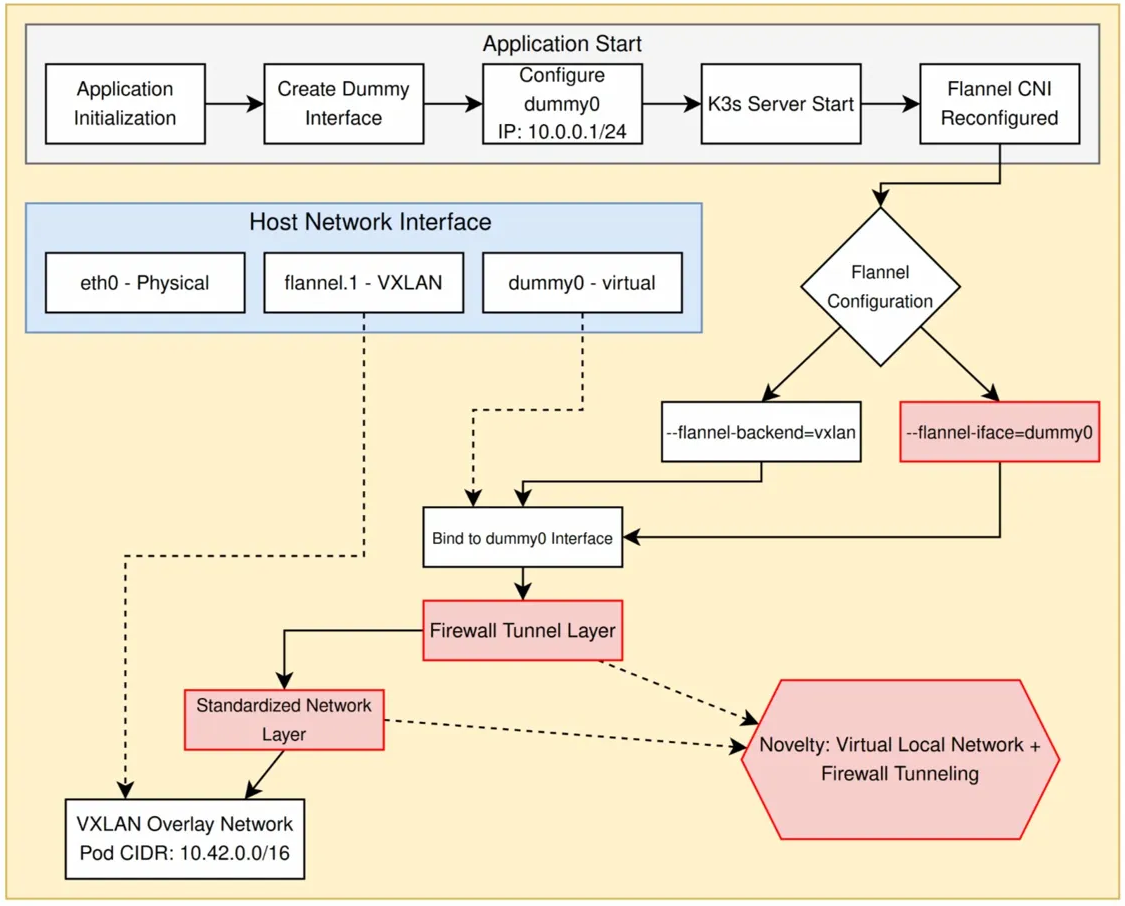
\includegraphics[width=0.75\linewidth]{images/inflection1.png}
    \caption{Inflection Point 1 resolution: Flannel CNI anchored to a virtual
\texttt{dummy0} interface rather than a physical network interface, decoupling
the K3s pod network from site firewall policies and producing a
site-agnostic VXLAN overlay (Pod CIDR 10.42.0.0/16).}
    \label{fig:inflection1}
\end{figure}

The result is a pod network that is entirely self-contained and site-agnostic. The same K3S configuration that works in the lab works at Stoutsville and at any future agricultural site, regardless of local firewall policy.

\subsection{The Hardware Had Other Plans}
\label{subsec:ch3_resource_contention}

\textbf{What happened.} A field laptop is not a cloud node. It has a fixed, constrained amount of RAM and CPU shared across the operating system, the K3S control plane, and every pod in the cluster. In the lab, the startup sequence presented no problem: containers initialized quickly on development hardware with headroom to spare. In Stoutsville, startup latency grew from the millisecond range to seconds. When multiple pods attempted to initialize simultaneously, the resource spike from their combined startup requirements exceeded what the edge laptop could supply. AI inference containers, which have larger initialization footprints than most workloads, crashed before completing their startup sequence. No inference, no orthomosaic, no output.

This failure mode is invisible in development because development environments have excess resources. The problem only surfaces when the total resource demand of simultaneous pod startups exceeds the available capacity of a single constrained node, which is exactly the condition that far-edge deployment creates.

\textbf{Why existing approaches did not cover this.} Standard Kubernetes scheduling assumes a multi-node cluster where pods can be distributed across nodes to balance load. K3S is single-node by design for far-edge use. Its default scheduler makes no accommodation for the simultaneous startup spike pattern. Pod Disruption Budgets exist in Kubernetes as a voluntary-disruption protection mechanism, specifically for administrator-initiated operations such as node drains and cluster upgrades, not for preventing OOM kills or crash-at-init failures during pod initialization.

%% P1.3 FIX: Two distinct mechanisms. Init container sequencing for crash-at-init. PDBs for protecting already-running pods.
\textbf{The solution: controlled startup sequencing with Pod Disruption Budget protection.} The response operates at two distinct levels, each addressing a different aspect of the resource contention problem.

At the initialization level, the crash-at-init failure is addressed through controlled pod startup sequencing. Rather than allowing all containers to race to initialize simultaneously, pods are sequenced using Kubernetes init containers and explicit resource requests. Init containers enforce an ordered startup dependency graph: resource-intensive pods do not begin initialization until their upstream dependencies have successfully started and released their initialization memory spike. Resource requests are configured explicitly for each pod so that the K3S scheduler has accurate information about each workload's startup footprint and can avoid overcommitting the node's capacity at any moment.

\begin{figure}
    \centering
    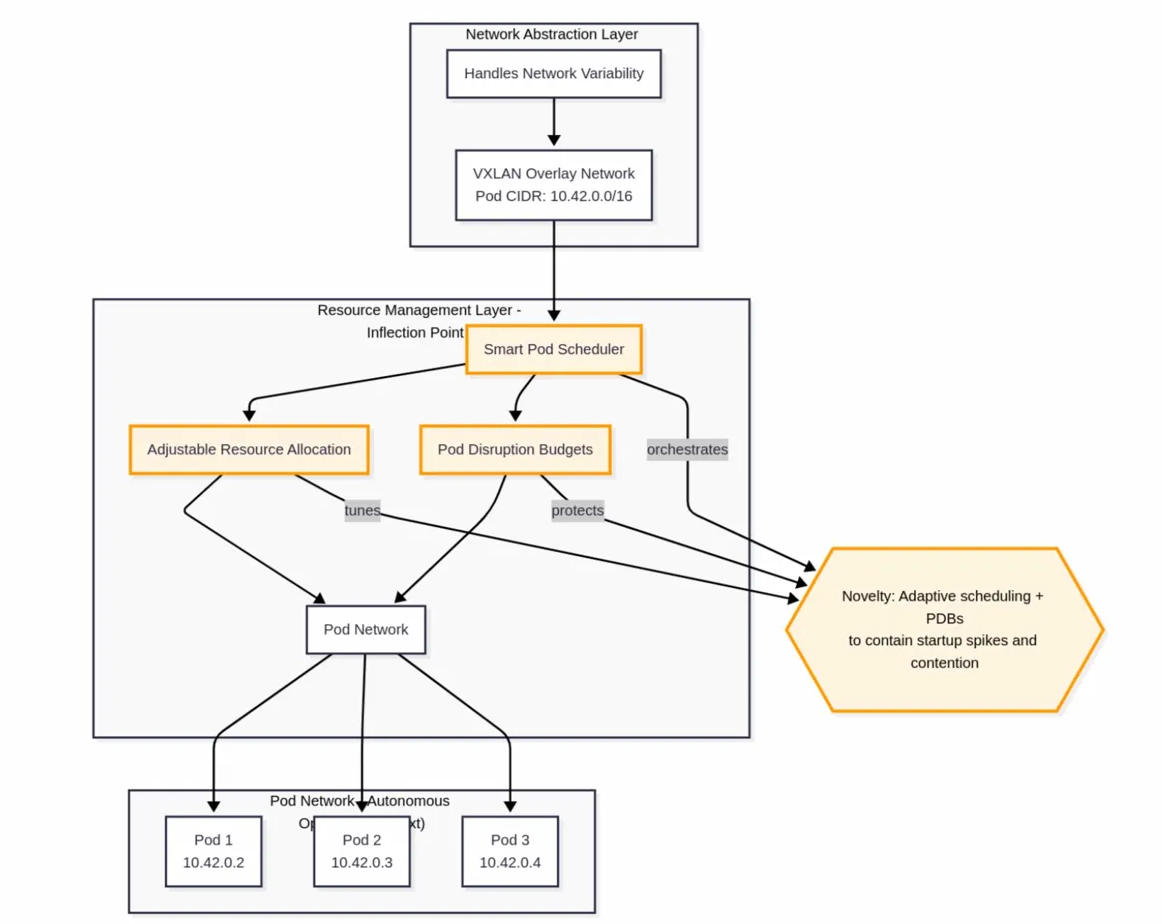
\includegraphics[width=0.75\linewidth]{images/inflection2.png}
    \caption{Inflection Point 2 resolution: init container sequencing enforces
ordered pod startup to prevent crash-at-init on constrained single-node
far-edge hardware; Pod Disruption Budgets protect already-running inference
pods from voluntary eviction during active missions.}
    \label{fig:inflection2}
\end{figure}

At the availability level, Pod Disruption Budgets are applied to the AI inference pods once they have entered a running state. PDBs are a Kubernetes mechanism for protecting already-running pods from voluntary disruptions such as node drains or administrator-initiated evictions. In the OpenPASS deployment, PDBs ensure that a running inference pod cannot be voluntarily evicted to free resources for other workloads during an active mission. These two mechanisms are complementary and target distinct failure modes: init container sequencing prevents crash-at-init; PDBs protect running inference pods from subsequent voluntary eviction.

The result is predictable startup behavior on constrained hardware. The edge node operates within its resource envelope at initialization, and inference pods are protected from eviction once running.

\subsection{No Registry, No Recovery}
\label{subsec:ch3_registry_dependency}

\textbf{What happened.} Agricultural fields at Stoutsville had zero network connectivity. This is not an edge case; it is the standard operating condition for working farm environments~\cite{elijah2018overview, wolfert2017bigdata}. The team had designed for local inference precisely because cloud access was not assumed. What had not been designed for was the behavior of K3S itself when connectivity was entirely absent.

Containerized applications built on standard cloud-native tooling carry a hidden dependency: the assumption that container images can be pulled from an external registry. This assumption is built into the operational model of containerd, the container runtime embedded in K3S. When a pod needs to be reconstructed, whether from a crash, a restart, or a fresh deployment, containerd attempts to pull the required image. If no registry is reachable, the pull fails, and the pod cannot be reconstructed.

\begin{figure}
    \centering
    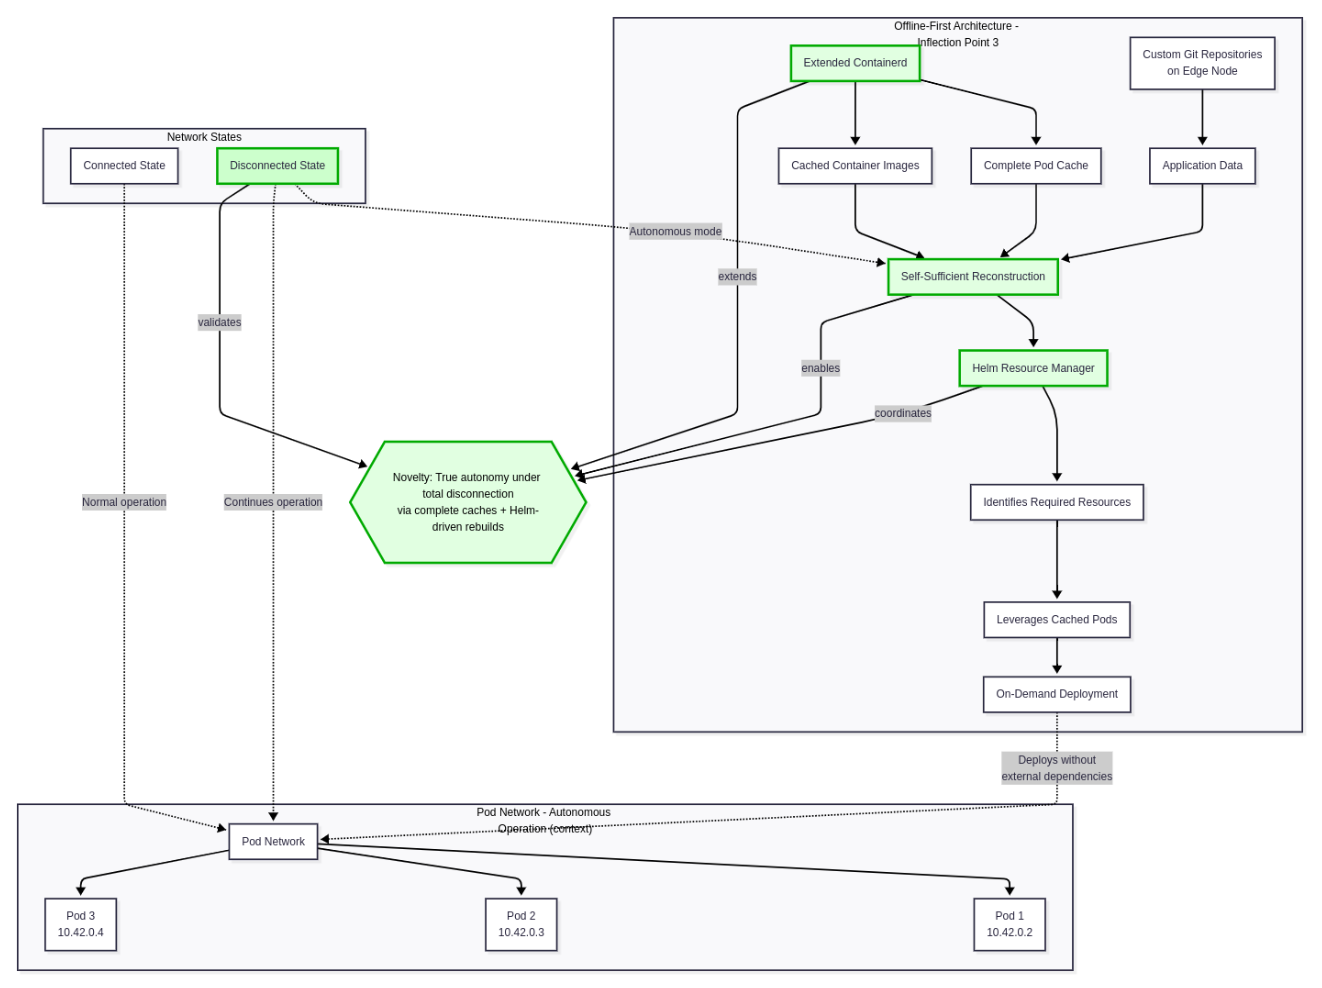
\includegraphics[width=0.75\linewidth]{images/inflection3.png}
    \caption{Inflection Point 3 resolution: air-gapped container image caches
and on-node Helm repositories enable self-sufficient pod reconstruction
under complete network disconnection; all chart and image dependencies
resolve from on-node storage with no external registry access required.}
    \label{fig:inflection3}
\end{figure}

In a lab or cloud environment, this failure mode never surfaces because registries are always reachable. In Stoutsville, it surfaced immediately. When pods crashed, they could not recover. When the team attempted a fresh deployment on-site, it failed. There was no recovery path without connectivity. This is the most consequential of the three inflection points because it makes far-edge deployment categorically different from near-edge or cloud deployment. The other two inflection points degrade performance. This one makes recovery impossible.

\textbf{Why existing approaches did not cover this.} K3S supports private registry mirroring through a \texttt{registries.yaml} configuration file, which redirects image pulls to a local mirror. However, this requires a registry service to be running and reachable on the local network. It is a redirection mechanism, not an offline cache. If the local registry is not running, K3S falls back to the external registry. OpenYurt and KubeEdge both inherit the same containerd-level dependency.

%% P1.4 FIX: Replace "extended containerd" with specific mechanism: ctr image import, registries.yaml, air-gapped deployment framing
\textbf{The solution: air-gapped image pre-population with local Helm repositories.} This solution operates at the configuration level, not the source level, and builds on a documented practice in the K3S and containerd communities known as air-gapped deployment~\cite{k3sdocs2024}.

All container images required by the OpenPASS application are pre-populated into containerd's local image store before the system leaves for the field, using \texttt{ctr image import} to load each image from archived tarballs stored on-node. A \texttt{registries.yaml} configuration in K3S is set to disable fallback to external registries, ensuring that containerd never attempts an outbound pull at runtime. When containerd resolves an image reference during pod reconstruction, it finds the image already present in the local store and serves it with no network request.

This is complemented by on-node Helm repository hosting. All Helm charts used by OpenPASS are stored in a local Git repository on the edge node. Helm operations resolve locally rather than against external chart repositories. The Helm Resource Manager coordinates pod rebuild sequences using only these local resources, reconstructing the full application stack from on-node storage alone.

Air-gapped deployment is a documented K3S practice~\cite{k3sdocs2024}. What this work adds is the diagnosis: runtime registry dependency functions as a structural failure mode in disconnected field missions, not an edge case. Combining that fix with the VXLAN overlay and startup sequencing produced the offline-first deployment pattern validated at Stoutsville.

The result is a system that self-reconstructs from a complete state of zero running pods, with no external network connectivity, using only what was loaded onto the node before deployment.

%% ============================================================
\section{A Framework for Deployment Failures}
\label{sec:ch3_framework}
%% ============================================================
The three inflection points encountered at Stoutsville are not specific to OpenPASS, to soybean fields, or to Ohio. They are instances of a general failure class that will appear in any far-edge AI deployment where the system was developed under cloud-native assumptions. The trigger conditions differ by site. The failure modes are consistent.

Table~\ref{tab:inflection_taxonomy} formalizes this as a structured taxonomy. Each entry documents the trigger condition, the failure mode it produces, and the architectural resolution that addresses it.

%% P1.2 FIX: Added \caption{} and \label{tab:inflection_taxonomy} so cross-reference resolves correctly
\begin{table}[htbp]
\centering
\small
\caption{Inflection-point taxonomy: trigger conditions, failure modes, and architectural resolutions for far-edge K3S deployments validated at Stoutsville, Ohio.}
\label{tab:inflection_taxonomy}
\begin{tabularx}{\textwidth}{|X|X|X|X|}
\hline
\textbf{Inflection Point} & \textbf{Trigger Condition} & \textbf{Failure Mode} & \textbf{Architectural Resolution} \\
\hline

Network Environment Mismatch
& Enterprise firewall blocks Flannel CNI's physical interface binding; UDP port 8472 unavailable
& Complete pod-to-pod communication failure; application non-functional at startup
& VXLAN overlay on virtual \texttt{dummy0} interface (standard Linux primitive, applied to K3s far-edge deployment); site-agnostic pod CIDR \texttt{10.42.0.0/16}; Flannel decoupled from physical network \\
\hline

Resource Contention at Startup
& Simultaneous pod initialization on constrained single-node edge hardware
& AI inference containers crash before completing initialization; no inference output
& Init container sequencing with explicit resource requests to prevent crash-at-init; Pod Disruption Budgets protecting already-running inference pods from voluntary eviction \\
\hline

Runtime Registry Dependency
& Zero network connectivity at deployment site; containerd attempts external image pull on pod reconstruction
& Complete application breakdown; no on-site recovery path without connectivity
& Air-gapped image pre-population via \texttt{ctr image import}; \texttt{registries.yaml} disabling external registry fallback; on-node Helm repositories for offline chart resolution \\
\hline

\end{tabularx}
\end{table}

We further propose an inflection-point database as a community artifact: a structured, shared repository where far-edge AI practitioners can document deployment failure modes, their trigger conditions, and their resolutions. Each entry follows the structure of Table~\ref{tab:inflection_taxonomy}. The goal is to reduce the rediscovery cost that every team currently bears when they carry a lab-validated system into a new physical environment. We are not aware of any equivalent structured repository in the far-edge AI literature. The proposed database described here is an invitation to the community, not a completed artifact.

%% ============================================================
\section{Validated Deployment and What It Demonstrated}
\label{sec:ch3_validated}
%% ============================================================
Following the resolution of all three inflection points, OpenPASS completed its mission at Stoutsville. The system deployed from on-node resources, established pod-to-pod connectivity through the VXLAN overlay, started its inference containers without resource contention failures, and operated through complete network disconnection without any loss of function.

%% P3.1 FIX: Added what the farmer received at end of a successful mission
The output of a completed mission was a georeferenced orthomosaic of the soybean field stitched from the drone's aerial survey pass, overlaid with a per-region crop health classification produced by the AI inference pipeline. This analysis was available to the farmer while the flight crew was still on-site: a color-coded field map indicating zones of stress, healthy growth, and anomalous readings, generated entirely on the field laptop without any data leaving the farm and without any network connectivity at any stage of the pipeline.

The architectural solutions validated at Stoutsville are not configurations written for one farm. They are a deployment pattern: a set of platform-level decisions that, taken together, make a K3S-based far-edge AI application resilient to the three infrastructure failure categories identified at Stoutsville. Each fix is domain-agnostic in its mechanism: the VXLAN overlay does not care about firewall policy; the init container sequencing applies to any constrained single-node hardware; the air-gapped pre-population holds wherever there is no connectivity. How far these principles transfer beyond digital agriculture is what Chapter 4 addresses.

That generality is the claim this thesis builds toward. This chapter established the pattern reactively, by encountering failures and resolving them. The question that follows is whether the same design principles, applied proactively, before any failure, on completely different hardware and in a completely different domain, produce the same resilience. Chapter 4 answers that question.